\documentclass[conference]{IEEEtran}
\IEEEoverridecommandlockouts
% The preceding line is only needed to identify funding in the first footnote. If that is unneeded, please comment it out.
\usepackage{float}
\usepackage{cite}
\usepackage{caption}
\usepackage{amsmath,amssymb,amsfonts}
% \usepackage{algorithmic}
\usepackage[dvipdfmx]{graphicx}
\usepackage{textcomp}
\usepackage{xcolor}
\usepackage{colortbl}
\usepackage[T1]{fontenc}
\usepackage{mdframed}
\usepackage{algorithm, algpseudocode} % texlive-science
\usepackage[braket, qm]{qcircuit}


\usepackage[braket, qm]{qcircuit}
\usepackage{tikz}
%
\newcommand*\rtofstarg{\tikz[baseline=(char.base)]{
            \node[shape=circle,double,draw,inner sep=1pt,minimum width=16pt] (char) {S};}}
\newcommand*\rtofsdgtarg{\tikz[baseline=(char.base)]{
            \node[shape=circle,double,draw,inner sep=1pt] (char) {S$^{\dagger}$};}}
\newcommand*\rtoftarg{\tikz[baseline=(char.base)]{
            \node[shape=circle,fill opacity=0,double,draw,inner sep=1pt] (char) {\phantom{S$^{\dagger}$}};}}
\newcommand*\rtofsctrl{\tikz[baseline=(char.base)]{
            \node[shape=circle,double,draw,inner sep=1pt,fill=black, minimum width=3pt] (char) {};}}
\newcommand*\rtofsctrlo{\tikz[baseline=(char.base)]{
            \node[shape=circle,double,draw,inner sep=1pt,fill=white, minimum width=3pt] (char) {};}}

\newcommand*\ctrlrtofs[1]{\push{\rtofsctrl}\qwx[#1]\qw}
\newcommand*\ctrlortofs[1]{\push{\rtofsctrlo}\qwx[#1]\qw}
\newcommand*\targrtofs{\push{\rtofstarg}\qw}
\newcommand*\targrtof{\push{\rtoftarg}\qw}

%\usepackage{floatrow}
\newtheorem{definition}{Definition}
\newtheorem{example}{Example}
\algrenewcommand\algorithmicindent{0.5em}%

\newcommand{\thickhline}{%
    \noalign {\ifnum 0=`}\fi \hrule height 1pt
    \futurelet \reserved@a \@xhline
}
%% \def\thickhline{%
%%   \noalign{\ifnum0=`}\fi\hrule \@height \thickarrayrulewidth \futurelet
%%   \reserved@a\@xthickhline}

%% \def\hlinewd#1{%
%% \noalign{\ifnum0=`}\fi\hrule \@height #1 %
%% \futurelet\reserved@a\@xhline}

\def\BibTeX{{\rm B\kern-.05em{\sc i\kern-.025em b}\kern-.08em
    T\kern-.1667em\lower.7ex\hbox{E}\kern-.125emX}}
\renewcommand{\baselinestretch}{1.11}
%\makeatletter
\newcommand{\figcaption}[1]{\def\@captype{figure}\caption{#1}}
\newcommand{\tblcaption}[1]{\def\@captype{table}\caption{#1}}
%\makeatother

\begin{document}

\title{Optimizing LUT-based Quantum Circuit Synthesis using Relative Phase Boolean Operations}
\author{\IEEEauthorblockN{\phantom{1\textsuperscript{st} David Clarino}}
  \IEEEauthorblockA{\phantom{\textit{Graduate School of}} \\
    \phantom{\textit{Information Science and Engineering}} \\
    \phantom{\textit{Ritsumeikan University}}\\
    \phantom{Kusatsu, Japan} \\
    \phantom{dizzy@ngc.is.ritsumei.ac.jp}}
  \and
  \IEEEauthorblockN{\phantom{2\textsuperscript{nd} Naoya Asada}}
  \IEEEauthorblockA{\phantom{\textit{Graduate School of }} \\
    \phantom{\textit{Information Science and Engineering}} \\
    \phantom{\textit{Ritsumeikan University}}\\
    \phantom{Kusatsu, Japan} \\
    \phantom{accel@ngc.is.ritsumei.ac.jp}}
  \and
  \IEEEauthorblockN{\phantom{3\textsuperscript{rd} Shigeru Yamashita}}
  \IEEEauthorblockA{\phantom{\textit{Graduate School of}} \\
    \phantom{\textit{ Information Science and Engineering}} \\
    \phantom{\textit{Ritsumeikan University}}\\
    \phantom{Kusatsu, Japan}\\
    \phantom{ger@ngc.is.ritsumei.ac.jp}}
}

\maketitle

\begin{abstract}
  LUT-based synthesis methods have recently been proposed as a way to
  synthesize quantum Boolean circuits in a qubit constrained
  environment. Other results have also shown that allowing a relative
  phase when implementing quantum Boolean circuits yields an advantage
  in T-count without additional ancilla qubits, which is advantageous
  in the fault-tolerant quantum computing paradigm. We propose a
  method that utilizes both LUT-based synthesis and relative phase
  quantum Boolean circuits that minimize the T-count while minimizing
  the ancilla required to implement them. We leverage recent results
  regarding relative phase versions of Boolean functions and the
  Shannon decomposition to propose a novel method to synthesize
  arbitrary Boolean functions up to a relative phase. We then utilize 
  this method to synthesize Boolean logic inside each LUT as a 
  relative phase quantum Boolean circuit and show that the resulting
  quantum circuit has a clear advantage in T-count to using it over 
  more naive methods.  
\end{abstract}

\begin{IEEEkeywords}
relative-phase Toffoli gates (RTOF), circuit optimization, LUT, synthesis
\end{IEEEkeywords}


      \begin{figure*}[hbt]
        \begin{minipage}{0.46\linewidth}
          \begin{center}
            % 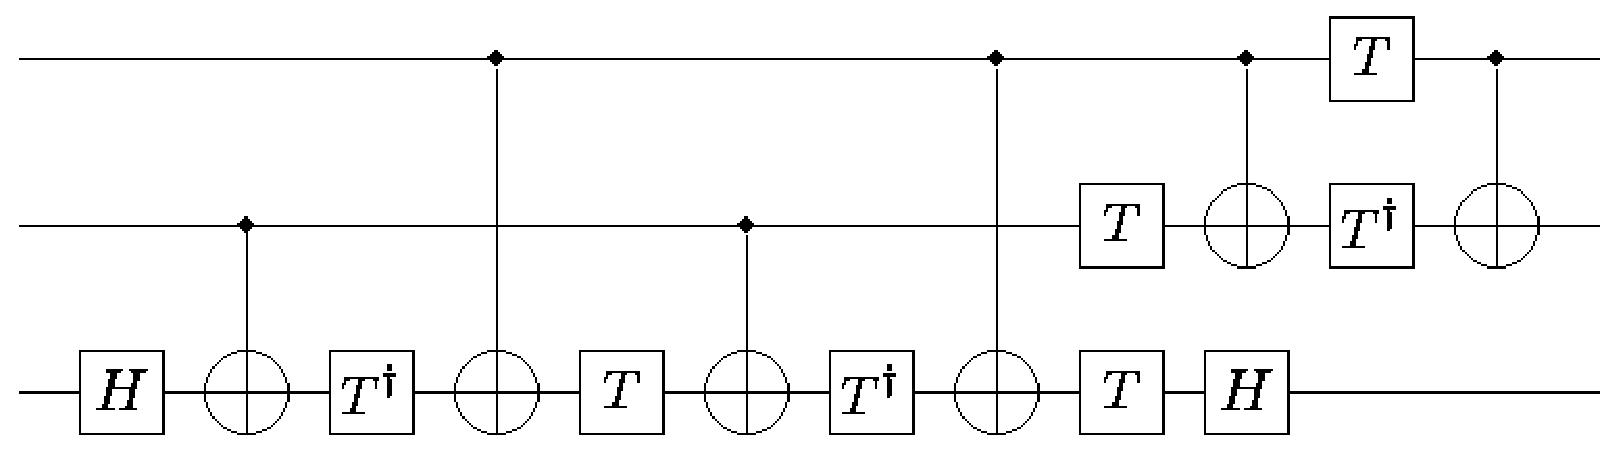
\includegraphics[width=6cm]{img/toffoli.eps}
           % 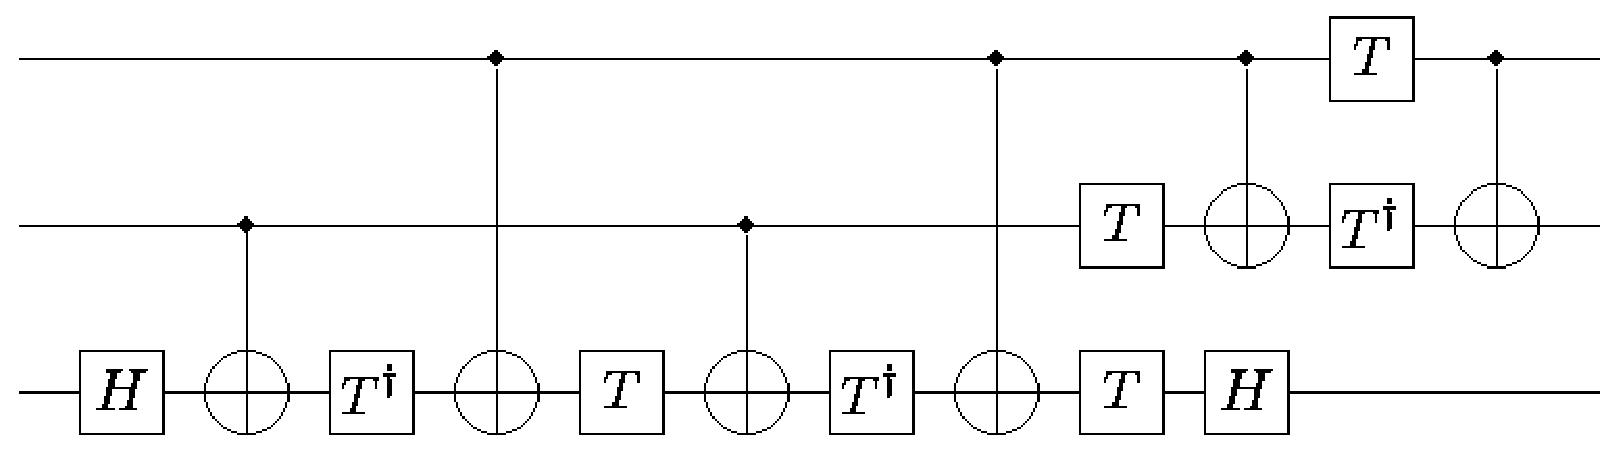
\includegraphics[width=\linewidth]{img/toffoli.eps}
            \Qcircuit @C=0.5em @R=0.2em @!R { \\
          \lstick{{x}_{0}} & \ctrl{2} & \qw &    & & \push{{x}_{0} :  } & \qw & \qw & \qw & \ctrl{2} & \qw & \qw & \qw & \ctrl{2} & \ctrl{1} & \gate{\mathrm{T}} & \ctrl{1} & \qw & \qw\\
          \lstick{{x}_{1}} & \ctrl{1} & \qw & \push{=}   & &\push{{x}_{1} :  } & \qw & \ctrl{1} & \qw & \qw & \qw & \ctrl{1} & \gate{\mathrm{T}} & \qw & \targ & \gate{\mathrm{T^\dagger}} & \targ & \qw & \qw\\
          \lstick{{f}}    & \targ \qw   & \qw &    & &  \push{{f} :  } & \gate{\mathrm{H}} & \targ & \gate{\mathrm{T^\dagger}} & \targ & \gate{\mathrm{T}} & \targ & \gate{\mathrm{T^\dagger}} & \targ & \gate{\mathrm{T}} & \gate{\mathrm{H}} & \qw & \qw & \qw\\
}

            \caption{A Toffoli gate in Clifford+T basis}
            \label{fig-toffoli}
          \end{center}
        \end{minipage}
        \hspace*{10mm}
        \begin{minipage}{0.46\linewidth}
          \begin{center}
            % \includegraphics[width=6cm]{img/rtof.eps}
            %\includegraphics[width=\linewidth]{img/rtof.eps}
            \Qcircuit @C=0.5em @R=0.2em @!R { \\
          \lstick{{x}_{0}} & \ctrl{2}\qw          & \qw &          & & \qw               & \qw               & \qw      & \qw                       & \ctrl{2} & \qw               & \qw      & \qw                         & \qw                &\qw\\
          \lstick{{x}_{1}} & \ctrl{1}             & \qw & \push{=} & & \qw               & \qw               & \ctrl{1} & \qw                       & \qw      & \qw               & \ctrl{1} & \qw                         & \qw                &\qw\\
          \lstick{{x}_{3}} & \push{\rtoftarg}\qw  & \qw &          & & \gate{\mathrm{H}} & \gate{\mathrm{T}} & \targ    & \gate{\mathrm{T^\dagger}} & \targ    & \gate{\mathrm{T}} & \targ    & \gate{\mathrm{T^{\dagger}}} & \gate{\mathrm{H}}  &\qw
}

            \caption{An RTOF gate in Clifford+T basis}
            \label{fig-rtof}
          \end{center}
        \end{minipage}
      \end{figure*}

    % ToffoliゲートとRTOFゲートの違いは，
    % RTOFゲートは入力によって回路の位相を変化させる場合があることにある．
    % 図\ref{rtof}に示すRTOFの全ての入力に対する位相は，表\ref{table-rtof}に示す通りである．
    % RTOFゲートの入力（$x_1, x_2, x_3$）が
    % $(1, 1, 0),(1, 0, 1), (1, 1, 1)$のとき，位相はそれぞれ，
      % $+\frac{\pi}{2}, +\pi, -\frac{\pi}{2}$だけ変化する．
\begin{figure*}[ht]
  \def\@captype{table}
  \begin{minipage}[ht]{.46\textwidth}
    \begin{center}
       %\scalebox{0.7}[1]{
        \begin{tabular}{c|c}      \hline
          input & $\Delta\theta$  \\\hline
          000   & 0      \\
          001   & 0      \\
          010   & 0      \\
          011   & 0      \\
          100   & 0      \\
          101   & $+\pi$          \\
          110   & $+\pi/2$   \\
          111   & $-\pi/2$ \\ \hline
        \end{tabular}        
    \end{center}
        \captionof{table}{Added phases by an RTOF.}
        \label{table-rtof}
  \end{minipage}
  \begin{minipage}[ht]{.46\textwidth}
    \begin{center}
      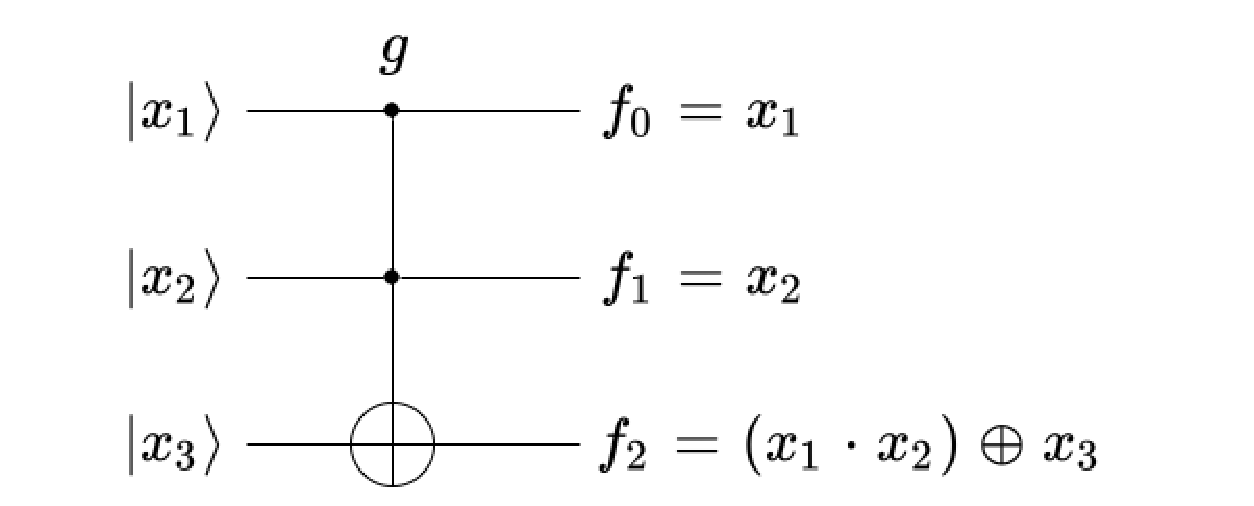
\includegraphics[width=5cm]{img/toffoli-f.eps}
      \caption{Functional representations for the output of a Toffoli gate.}
      \label{toffoli-f}
    \end{center}
  \end{minipage}

  
  %
 \end{figure*}

\section{Introduction}

Boolean functions are often used as essential components in quantum algorithms, such as oracles and cost functions; these are often calculated using the circuit model called {\it quantum Boolean circuits}~\cite{bib-circuit}. To realize such quantum Boolean circuits, a Toffoli gate is often used as a logic primitive. However, as three qubit operations do not occur naturally in the two level systems that modern quantum computers are made of, these Toffoli gates have to be in turn, composed of physically realizable gates, such as NOT, CNOT, and T. (e.g., the Clifford+T~\cite{bib-gates} basis gate set), as depicted in Fig.~\ref{toffoli}

As qubits are famously prone to error and perturbation, it is often useful to consider a {\it fault-tolerant} implementation of quantum computation, one which could detect and correct errors ~\cite{bib-mike-and-ike}. Unfortunately, in the fault-tolerant paradigm, T-gates incur much higher cost than so-called Clifford gate types. Many of the most prominent implementations employ state purification and gate teleportation, among others. Because of its relatively outsized cost compared to Clifford gates, it has the possibility of overwhelming the base cost of a particular circuit implementation. As T gates are key to quantum advantage, due to the Gottesman-Knill Theorem, decreasing the number of T-gates (T-count) has been identified as of paramount importance in bridging the gap between theoretical models of quantum computation and their physically realizable counterparts, and many propositions have been made to decrease their number in a given circuit.

Our research seeks to leverage recent results in relative phase implementations of Boolean functions ~\cite{bib-rtof-maslov} ~\cite{bib-amy-phase-state} and LUT-based quantum circuit synthesis to reduce T-count in a a qubit constrained environment.

\noindent {\bf Our Contribution.} 
We propose a method that reduces the number of T-gates in a Quantum LUT Network by exploiting relative phase Boolean functions. Among our contributions:
\begin{itemize}
\item A novel method to synthesize a Boolean function up to a relative phase by utilizing relative phase constructions and Shannon Decomposition
\item A method to generate a Quantum Boolean Circuit from a Boolean Logic Network representation leveraging the above method to reduce T-count

\end{itemize}
Our methods are compared to a naive synthesis of each LUT node that utilizes an ESOP-based method to synthesize each Boolean function exactly as a Quantum Boolean Circuit. We find that on average, for similar usage of ancilla qubits, this improves T-count by DCTODO\%. While there remain a few exceptions to its advantage, its advantage in the majority of cases we have tested points to more resea

The paper is structured as follows. Section~\ref{Sec:prelim} outlines preliminary information for understanding this paper. Then Section~\ref{Sec:Exist} lays out some motivations for the research we are going to conduct. Section~\ref{Sec:proposed} follows with our proposed method, including our novel method to realize functions up to a relative phase without any additional ancillae, and then its use with the LHRS. Then, Our experimental results in Section~\ref{Sec:exp} can confirm that our method can indeed reduce the T-count of quantum Boolean circuits. Finally Section~\ref{Sec:concl} concludes the paper with our conclusions and future work.


\begin{figure}[tbp]
  \begin{center}
    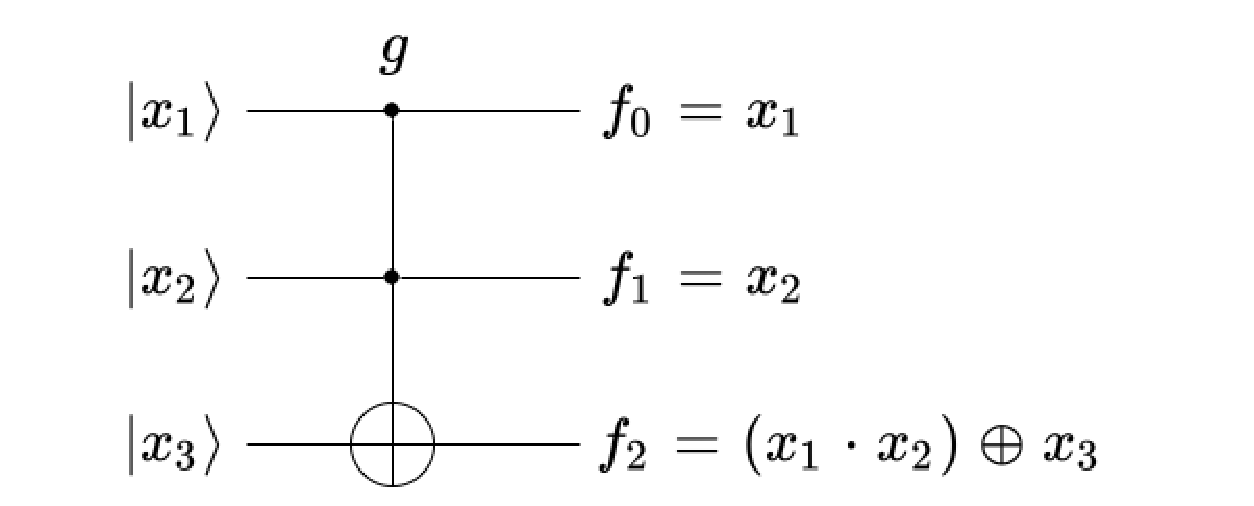
\includegraphics[width=5cm]{img/toffoli-f.eps}
    \caption{Functional representations for the output of a Toffoli gate.}
    \label{toffoli-f}
  \end{center}
  %\vspace*{-1cm}
\end{figure}
\begin{figure}[t]
  \label{fig-bool-or}
\end{figure}
\begin{figure}[t]
  \label{fig-bool-and}
\end{figure}


\section{Preliminary}
\label{Sec:prelim}
\subsection{Quantum Boolean Circuits}

In this paper, we consider {\it quantum Boolean circuits}~\cite{bib-ddmf} that implement Boolean functions, consisting of Toffoli gates, T gates, S gates and relative-phase Toffoli gates (RTOFs)~\cite{bib-rtof}. 

We denote the primary inputs of a circuit by $x_1, x_2, \cdots,x_{n}$  when we have $n$ primary inputs. Each qubit state in a circuit consisting of Toffoli and RTOF gates can be represented by a Boolean function with respect to $x_1, x_2, \cdots,x_{n}$.

 \subsection{Boolean Constructions}
 \label{Sec:bool-const}
We will be using a few common constructions to realize certain Boolean operations as quantum circuits. Fig.~\ref{fig-bool-or} depicts how putting the output of two Toffoli or CNOT gates in series on the same output qubit will create a Boolean sum of their controls, while ~\ref{fig-bool-and} depicts how putting their outputs in parallel on the controls of a Toffoli gate will produce their Boolean product on the Toffoli gate's output (assuming a clean ancilla). We will be using these facts in the next section. 

\subsection{Relative-Phase Toffoli Gates (RTOFs)}

An RTOF (Relative-Phase Toffoli) gate~\cite{bib-rtof} has two control bits and one target bit. It inverts the basis state of the target bit (i.e., $\ket{1}$ to $\ket{0}$ and $\ket{0}$ to $\ket{1}$) when the states of the both control bits are $\ket{11}$. A Toffoli gate consists of 7 T gates as shown in Fig.~\ref{toffoli} whereas an RTOF consists of 4 T gates as shown in Fig.~\ref{rtof}. One may notice that the version of the RTOF that is used here is similar to the n-controlled-iX gate from ~\cite{bib-selinger-rtof} for $n=2$, with one less CNOT gate. As noted in ~\cite{bib-rtof}, removing this gate only affects the phase, so it only transforms an RTOF gate into another RTOF gate. We will subsume this

As depicted in Fig.~\ref{rtof}, an RTOF has three inputs; the input quantum basis states are $\ket{000}$ to $\ket{111}$. Similar to Toffoli gates, an RTOF swaps  $\ket{110}$ and $\ket{111}$. In addition to this logic operation, RTOF gates add phases to some output states that the equivalent Toffoli gate does not. The added phases are as shown in Table~\ref{table-rtof}. For example, when the input state is $\ket{110}$, a phase $+\pi/2$ is added.

One of the results from ~\cite{bib-rtof} is that when larger functions are broken down into compute/uncompute pairs, such as in the Barenco style Toffoli decompositions, it is almost always more advantageous to implement each ``half'' of the compute/uncompute pair into a relative phase construction. We will next go into one such construction.

\subsection{Relative-Phase Boolean Functions}

As an extension of the RTOF

\subsection{Boolean Logic Network}

A {\it Boolean Logic Network} is a simple dag whose vertices are primary inputs, primary outputs, and nodes which represent logic gates, whose arcs connect gates to inputs, outputs, and other gates.

A node {\it n} has zero or more {\it fanins}, or incoming edges, and zero or more {\it fanouts} i.e. outgoing edges. The {\it primary inputs (PIs)} are nodes without fanins in the current network. The {\it primary outputs} are a subset of nodes of the network without fanouts. 

A logic function can be decomposed into such a Boolean Logic Network, and its nodes subsequently implemented as LUTs or logic gates.

 \section{Existing Research}
 \label{Sec:Exist}
\subsection{LUT-based Hierarchical Reversible Logic Synthesis (LHRS)}
\label{Sec:lhrs}
Previous Research ~\cite{bib-soeken2018lut} has detailed a way to leverage LUT-based synthesis of Boolean functions to create reversible logic networks that will be essential to quantum Boolean circuits. The overall flow maps each node in the Boolean Network to a function-controlled NOT gate, and then cascades them together to create the output. Because the U-controlled NOT gates act on ancillas, there is a need to uncompute them, so the flow next produces uncompute logic. This produces the compute/uncompute pair that a relative-phase based construction of the function can take advantage of. 

\subsection{Using RTOF to decompose MCT gates}
Existing research ~\cite{bib-rtof} finds an advantage to using RTOFs in synthesizing and decomposing logic functions, particularly MCTs. For the sake of brevity, we will only detail their results here that we will use.
\begin{itemize}
\item Replacing pairs of computing and uncomputing gates with RTOF and its inverse will lead to T gate savings in most cases
\item Using the above, it is possible to use clean-ancilla to decompose an MCT with fewer T gates than the known methods.
\item A recursive procedure to generate MCT gates up to a relative phase
\end{itemize}
%%% Local Variables:
%%% mode: japanese-latex
%%% TeX-master: "main"
%%% End:

%% \begin{figure}
%%   \label{fig-maslov-decomp}
%% \end{figure}
\begin{figure}[ht]
  \begin{minipage}{.46\textwidth}
    \begin{center}
      \usetikzlibrary{positioning}
\definecolor{offwhite}{HTML}{F2EDED}
%% \tikzset{
%%     > = stealth,
%%     every node/.append style = {
%%         draw = none,
%%         text = offwhite
%%     },
%%     every path/.append style = {
%%         arrows = ->,
%%         draw = offwhite,
%%         fill = offwhite
%%     },
%%     hidden/.style = {
%%         draw = offwhite,
%%         shape = circle,
%%         inner sep = 1pt
%%     }
%% }
%% \tikz{
%%     \node (x) {$X$};
%%     \node[hidden] (z) [above right = of x] {$Z$};
%%     \node (y) [below right = of z] {$Y$};
%%     \path (x) edge (y);
%%     \path (z) edge (x);
%%     \path (z) edge (y);
%% }
\tikzset{
  > = stealth,
  every node/.append style = {
    draw      = offwhite,
    shape     = circle,
    inner sep = 1
  },
  every path/.append style = {
        arrows = ->,
        draw = offwhite,
        fill = offwhite
  },  
  input/.style = {
    draw = none
  }
}

\tikz{
  \node[input] (x1) at (0,0) {$x1$};
  \node[input] (x2) at (1,0) {$x2$};
  \node[input] (x3) at (2,0) {$x3$};
  \node[input] (x4) at (3,0) {$x4$};
  \node[input] (x5) at (4,0) {$x5$};
  \node[input] (y1) at (1,3) {$y1$};
  \node[input] (y2) at (3,4) {$y2$};
  \node (1) at (1,1) {$1$};
  \node (2) at (3,1) {$2$};
  \node (3) at (1,2) {$3$};
  \node (4) at (3,2) {$4$};
  \node (5) at (3,3) {$5$};      
  \path (x1) edge (3);
  \path (x2) edge (1);
  \path (x3) edge (1);
  \path (x4) edge (1);
  \path (x4) edge (2);
  \path (x5) edge (2);
  \path (x5) edge (5);
  \path (1)  edge (3);
  \path (1)  edge (4);    
  \path (2)  edge (4);
  \path (4)  edge (5);
  \path (3)  edge (y1);
  \path (5)  edge (y2);  
}

      \label{fig-lut_network}
      \caption{A Boolean Logic Network}

    \end{center}
  \end{minipage}
  \begin{minipage}{0.46\textwidth}

    \begin{center}
      \Qcircuit @C=0.5em @R=0.2em @!R { \\
  \lstick{\ket{{x}_{1}}} & \qw  & \qw               & \qw               & \multigate{5}{3} & \qw                & \qw              & \qw                        & \qw                        & \qw                         & \ghost{x_1}  \\
  \lstick{\ket{{x}_{2}}} & \qw  & \multigate{1}{1}  & \qw               & \ghost{3}\qw     & \qw                & \qw              & \qw                        & \qw                        & \multigate{1}{1^{\dagger}}  & \ghost{x_2}  \\
  \lstick{\ket{{x}_{3}}} & \qw  & \ghost{1}         & \qw               & \ghost{3}\qw     & \qw                & \qw              & \qw                        & \qw                        & \ghost{1^{\dagger}}         & \ghost{x_3}  \\
  \lstick{\ket{{x}_{4}}} & \qw  & \qw               & \multigate{1}{2}  & \ghost{3}\qw     & \qw                & \qw              & \qw                        & \multigate{1}{2^{\dagger}} & \qw                         & \ghost{x_4}  \\
  \lstick{\ket{{x}_{5}}} & \qw  & \qw               & \ghost{2}         & \ghost{3}\qw     & \qw                & \multigate{3}{5} & \qw                        & \ghost{2^{\dagger}}        & \qw                         & \ghost{x_5}  \\
  \lstick{\ket{0}     }  & \qw  & \targ\qwx[-3]\qw  & \qw               & \ghost{3}\qw     & \multigate{1}{4}   & \ghost{5}        & \multigate{1}{4^{\dagger}} & \qw                        & \targ\qwx[-3]\qw            & \ghost{0}      \\
  \lstick{\ket{0}     }  & \qw  & \qw               & \targ\qwx[-2]\qw  & \targ\qwx[-1]\qw & \ghost{4}          & \ghost{5}        & \ghost{4^{\dagger}}        & \targ\qwx[-2]\qw           & \qw                         & \ghost{y_1}  \\
  \lstick{\ket{0}     }  & \qw  & \qw               & \qw               & \qw              & \targ\qwx[-1]\qw   & \ghost{5}        & \targ\qwx[-1]\qw           & \qw                        & \qw                         & \ghost{0}      \\
  \lstick{\ket{0}     }  & \qw  & \qw               & \qw               & \qw              & \qw                & \targ\qwx[-1]\qw & \qw                        & \qw                        & \qw                         & \ghost{y_2}  \\
}

      \caption{The Boolean Quantum Circuit implementing Fig. \ref{fig-lut_network} }
      \label{fig-lut-network}
    \end{center}
  \end{minipage}

\end{figure}


\section{Existing Research and Motivation}

Because not all Boolean functions can be implemented as unitaries, from the very early days of Quantum Computing~\cite{bib-barenco-elementary}, it has been known that in addition to adding ancilla to the circuit to store temporary values, allowing the final states to have differing phases ({\it relative phase}) with respect to each other is also a valid way to implementa Boolean function.

Relative phase versions of quantum operations, such as the {\it Relative-phase Toffoli gates (RTOF)}~\cite{bib-rtof-maslov} ~\cite{bib-selinger-rtof} have been proposed as an alternative . One of the proposed implementations of the RTOF depicted in Fig. ~\ref{fig-rtof} can calculate the same logic function as a Toffoli gate and reduces the T-gate count by 3. However it introduces a {\it relative phase} among its output quantum states, (enumerated in Table ~\ref{table-rtof}. Because of the introduced relative phase, we cannot simply replace a Toffoli gate with an RTOF in general. Rather, RTOFs can be utilized when we decompose a multiple-control Toffoli gate because the relative phase errors can be canceled between two RTOFs in the decomposition ~\cite{bib-rtof-maslov}.

Maslov further posits that not just Toffoli gates but generalized controlled U functions can take advantage of the fact that Boolean functions implemented up to a relative phase used in tandem can optimize the overall circuit.

Meanwhile, LUT-based quantum circuit synthesis has been proposed as a way to synthesize quantum circuits in an environment where available clean ancillae for use as intermediate qubits is limited. Methods such as the LHRS ~\cite{bib-lhrs-soeken}  synthesize each of these LUTs is implemented as a U-controlled NOT function. Naturally, this leads to a cascading series of gates, along with their uncompute pairs. This structure naturally lends itself to the construction from Maslov, where alternating pairs of gates can cancel their relative phases.

In light of these facts, it is easy to imagine a method that utilizes relative phase Boolean functions to reduce the cost of gates in the LUT network, all while adding no additional ancillae. The key will be a method to generate relative phase Quantum Boolean Circuits from arbitrary Boolean functions. We propose such a method in this work.




\begin{figure}[t]
  \label{fig-rtof3}
\end{figure}
\begin{figure}[t]
  \label{fig-nrtof}
  \begin{center}
    \Qcircuit @C=0.5em @R=0.2em @!R { \\
          \push{{x}_{0} } & \qw               & \qw                     & \qw      & \qw                      & \control{2}\qw\qwx[1] & \qw                & \qw      & \qw                       & \qw \\
          \push{{x}_{1} } & \qw               & \qw                     & \qw      & \qw                      & \control{2}\qw\qwx[1] & \qw                & \qw      & \qw                       & \qw \\
          \push{\vdots}   &                   &                         &          &                          & \push{\vdots}          &                    &          &                           & \push{\vdots} \\
          \push{{x}_{n} } & \qw               & \qw                     & \ctrl{1} & \qw                      & \qw                   & \qw               & \ctrl{1}  & \qw                       & \qw \\
          \push{{f}   }  & \gate{\mathrm{H}} & \gate{\mathrm{T^\dagger}} & \targ     & \gate{\mathrm{T^\dagger}} & \targ\qwx[-1]         & \gate{\mathrm{T}} & \targ     & \gate{\mathrm{T^{\dagger}}} & \gate{\mathrm{H}} \\
}

  \end{center}
  \caption{N-controlled RTOF gate}
\end{figure}
\begin{figure}[t]
  \label{fig-urtof}
  \begin{center}
    \Qcircuit @C=0.5em @R=0.2em @!R { \\
          \push{{x}_{0} }   & & \multigate{3}{x_k \cdot U}  & \qw   & \qw & &         & & \qw & \qw               & \qw                       & \qw      & \qw                       & \multigate{3}{U}              & \qw               & \qw      & \qw                         & \qw               & \qw & \\
          \push{{x}_{1} }   & & \ghost{x_k \cdot f}         & \qw   & \qw & &         & & \qw & \qw               & \qw                       & \qw      & \qw                       & \ghost{U}                      & \qw               & \qw      & \qw                         & \qw               & \qw & \\
          \push{\vdots}     & &                             &       &     & &\push{=} & &     &                   & \push{\vdots}             &          &  \push{\vdots}            &                                & \push{\vdots}     &          &                             & \push{\vdots}     &     & \\
          \push{{x}_{n-1} } & & \ghost{x_k \cdot f}         & \qw   & \qw & &         & & \qw & \qw               & \qw                       & \ctrl{1} & \qw                       & \ghost{U}                      & \qw               & \ctrl{1} & \qw                         & \qw               & \qw & \\
          \push{{x}_{n} }   & & \push{\rtoftarg}\qw\qwx[-1] & \qw   & \qw & &         & & \qw & \gate{\mathrm{H}} & \gate{\mathrm{T}}         & \targ    & \gate{\mathrm{T^\dagger}} & \targ\qwx[-1]    & \gate{\mathrm{T}} & \targ    & \gate{\mathrm{T^{\dagger}}} & \gate{\mathrm{H}} & \qw & \rstick{e^{i\phi(x_0,\ldots,x_n)} \ket{x_n \cdot U(x_0, \ldots,x_{n-1}) + \phi_{U*}} } \\
}
                            

  \end{center}
  \caption{U-controlled RTOF gate}
\end{figure}
\begin{figure}[t]
  \label{fig-f-dot-g}
  \begin{center}
    \Qcircuit @C=0.5em @R=0.2em @!R { \\
          \push{{x}_{0} }    & & \multigate{5}{x_k \cdot U}  & \qw   & \qw & &         & & \qw               & \qw                       & \qw      & \qw                       & \multigate{5}{U}                & \qw               & \qw      & \qw                         & \multigate{5}{U^{\dagger}}       & \qw              & \qw & \\
          \push{{x}_{1} }    & & \ghost{x_k \cdot f}         & \qw   & \qw & &         & & \qw               & \qw                       & \qw      & \qw                       & \ghost{f}                       & \qw               & \qw      & \qw                         & \ghost{f}                        & \qw              & \qw & \\
          \push{\vdots}      & &                             &       &     & &\push{=} & &                    & \push{\vdots}            &          &  \push{\vdots}            &                                 & \push{\vdots}     &          &                             &                                  & \push{\vdots}    &     & \\
          \push{{x}_{k} }    & & \ghost{x_k \cdot f}         & \qw   & \qw & &         & & \qw               & \qw                       & \ctrl{3} & \qw                       & \ghost{f}                       & \qw               & \ctrl{3} & \qw                         & \ghost{f}                        & \qw              & \qw & \\
          \push{\vdots}      & &                             &       &     & &\push{=} & &                    & \push{\vdots}            &          &  \push{\vdots}            &                                 & \push{\vdots}     &          &                             &                                  & \push{\vdots}    &     & \\
          \push{{x}_{n} }    & & \ghost{x_k \cdot f}         & \qw   & \qw & &         & & \qw               & \qw                       & \qw      & \qw                       & \ghost{f}                       & \qw               & \qw      & \qw                         & \ghost{f}                        & \qw              & \qw & \\
          \push{{\ket{0}}   }& & \push{\rtoftarg}\qw\qwx[-1] & \qw   & \qw & &         & & \gate{\mathrm{H}} & \gate{\mathrm{T^\dagger}} & \targ    & \gate{\mathrm{T^\dagger}} & \push{\rtoftarg}\qw\qwx[-1]     & \gate{\mathrm{T}} & \targ    & \gate{\mathrm{T^{\dagger}}} & \push{\rtoftarg}\qw\qwx[-1]\qw   &\gate{\mathrm{H}} & \qw & \rstick{e^{i\phi(x_0,\ldots,x_n)} \ket{x_k \cdot U(x_0, \ldots,x_{n-1})} }\\
}


  \end{center}
  \caption{Generalization of Fig.\ref{fig-urtof}, which also implements the Boolean product of two functions}
\end{figure}
\begin{figure}[t]
  \label{fig-shannon}
\end{figure}


\section{Proposed Method}

\subsection{Realizing Arbitrarily Controlled NOT Functions Up To A Relative Phase}
\label{Subsec:UNOT}
To get to a point where we can realize arbitrary Boolean functions up to a relative phase, we first observe that the RTOF gate depicted in Fig.~\ref{fig-rtof} can replace the center CNOT with a n-input Toffoli gate as depicted in Fig.~\ref{fig-nrtof} which was observed by Maslov ~\cite{bib-rtof-maslov}. As noted by Maslov, we can ostensibly continue this indefinitely for n-input Toffoli gates until we arrive at a canonical 3 input example. We can generalize this n-input Toffoli to an arbitrarily controlled NOT gate as depicted in ~\ref{fig-urtof}. It is easy to see this without further proof: we can imagine implementing the Boolean function separately and then routing its input to an input bit via a clean ancilla.

We can further generalize this. Recall from \label{Sec:bool-const} that a Toffoli realizes a Boolean product of its inputs on its output. Just like above, we can use the same reasoning to generalize both inputs into arbitrary Boolean functions ~\cite{bib-amy-phase-state} . This means that we can use the construction in ~\ref{fig-f-dot-g} to realize a product between two arbitrary Boolean functions up to a relative phase. 


\subsection{Using Shannon Decomposition To Realize Arbitrarily Controlled Single Target Gates}

Recall the Shannon Decomposition $f(x_n,...,x_1) = x_n \cdot f(x_n=1,x_{n-1},\cdots,x_0) + \bar{x_n} \cdot f(x_n=0,x_{n-1},\cdots,x_0)$. Using the constructions in ~\ref{Subsec:UNOT}, we thus have a way to recursively construct arbitrary Boolean Functions up to a relative phase as a single target controlled NOT gate.

First, from the Shannon decomposition $f(x_n,...,x_1) = x_n \cdot f(x_n=1,x_{n-1},\cdots,x_0) + \bar{x_n} \cdot f(x_n=0,x_{n-1},\cdots,x_0)$ where we can take $g=f(x_n=1,x_{n-1},\cdots,x_0)$ and $g^{\prime}=f(x_n=0,x_{n-1},\cdots,x_0)$\footnote{note that as with any Shannon decomposition, we can decompose using an arbitrary variable order. We will treat variable order in ~\ref{Sec:exp}}. We then take ~\ref{fig-bool-or} and replace the inputs with our inputs, and the Toffoli gates with RTOFs (and their decomposition). Finally, we take ~\ref{fig-f-dot-g} to insert our function, and we get the construction in Fig.~\ref{fig-shannon}. As noted in ~\ref{Subsec:UNOT}, it is easy to see that this expression implements the Sum of Products (SOP) expression of the Shannon decomposition. We then take each of $g$ and $g^{\prime}$ and repeat the process until we are left with a simple CNOT as our U-controlled NOT expression. 

\begin{example}
  
\end{example}

\subsection{Synthesizing A Boolean Function Using LHRS and Shannon Decomposition RTOF}

First, a LUT network is synthesized from the Boolean expression using existing LUT-Network decomposition methods, including any uncomputation logic. Then, this LUT network is parsed by our algorithm, creating quantum circuits implementing relative phase versions of the partial Boolean functions in each cluster with an uncompute pair, and exact versions in each cluster (using an ESOP-based synthesis method) without an uncompute pair. These are then recombined into a quantum circuit

\section{Experimental Results}

\subsection{Methodology}

Boolean functions are taken from benchmarks and fed into the abc tool \cite{bib-abc} which generates a LUT-network with LUT size of at most 6 variables. This LUT network is then parsed according to LHRS and converted to a quantum circuit implemented in Qiskit ~\cite{bib-qiskit}. The Shannon Decomposition algorithm uses the Tulip Control BDD library ~\cite{bib-tulip-dd} to implement its Boolean functions, as well as reorder the variables for optimality. Because the variables are limited to 6, we use an exhaustive search to determine the optimal variable order. Any exact synthesis of Boolean functions is conducted using Qiskit's ClassicalFunction functionality, which uses the ESOP-based PKRM algorithm ~\cite{bib-pkrm}.

The results are compared the LHRS method in ~\cite{bib-lhrs-soeken}, using ClassicalFunction as the ESOP-based synthesis method to implement the LUT functions to approximate their method.

\begin{table*}[t]
  \large
   \begin{center}
     \caption{Experimental Results}
     \scalebox{0.7}{
       \begin{tabular}{c|c|c}
         \hline
        Circuit\_Name & Proposed & LHRS\\ \hline
        priority\_size\_2022 & 3888 & 17340 \\
        int2float\_size\_2022 & 2684 & 4516 \\
        i2c\_size\_2022 & 9388 & 16432\\
        dec\_size\_2018 & 10084 & 18100\\
        ctrl\_size\_2022 & 2088 & 2576\\
        cavlc\_size\_2022 & 8976 & 20764\\
        bar\_size\_2015 & 139168 & 42808\\
        arbiter\_size\_2022 & 8076 &  30916 \\
        adder\_size\_2022 &11248 & 1624 \\\hline
       \end{tabular}
     }
     \label{table-results}
     \end{center}
\vspace*{0.25cm}
 \end{table*}







\section{Conclusion}
\label{Sec:concl}
This paper proposed the use of relative phase Boolean functions to optimize LUT-based quantum circuit synthesis while maintaining a minimum of ancillae. While the Shannon decomposition allows us to the cost remains exponential with respect to the number of LUT inputs, limiting the LUT-size to 6 still allows us to see a significant T-count advantage in the proposed method. There still remain some cases where it underperforms the naive case so further research will be needed there. Furthermore, it remains an open question whether we can get better than exponential cost for the LUTs. As shown in ~\cite{bib-soeken-lhrs}, increasing LUT size has possible advantages in gate count and depth. There remain many possible paths this research can be taken along.


%\renewcommand{\baselinestretch}{1.2}
\vspace{0.1cm}
\renewcommand{\baselinestretch}{1.06}
\bibliographystyle{plain}
\bibliography{ref}
%\vspace{12pt}
\end{document}
